\fancyhead[LO]{{\scriptsize {\FA \ }我们最幸福 {\FA } 不洁之血}}%奇數頁眉的左邊
\fancyhead[RO]{{\tiny{\textcolor{Gray}{\FA \ }}}\thepage}
\fancyhead[LE]{{\tiny{\textcolor{Gray}{\FA \ }}}\thepage}
\fancyhead[RE]{{\scriptsize {\FA \ }我们最幸福 {\FA } 不洁之血}}%偶數頁眉的右邊
\fancyfoot[LE,RO]{}
\fancyfoot[LO,CE]{}
\fancyfoot[CO,RE]{}
\chapter*{02 {\FA } 不洁之血}
\addcontentsline{toc}{chapter}{\hspace{5mm}02 \textbf{>}\ \ 不洁之血}
\vspace{5mm}
\begin{flushright}
	\textcolor{PinYinColor}{\EN \huge{Tainted\\
		Blood\\
	\ \\}}
\end{flushright}
\begin{figure}[!htbp]
	\centering
	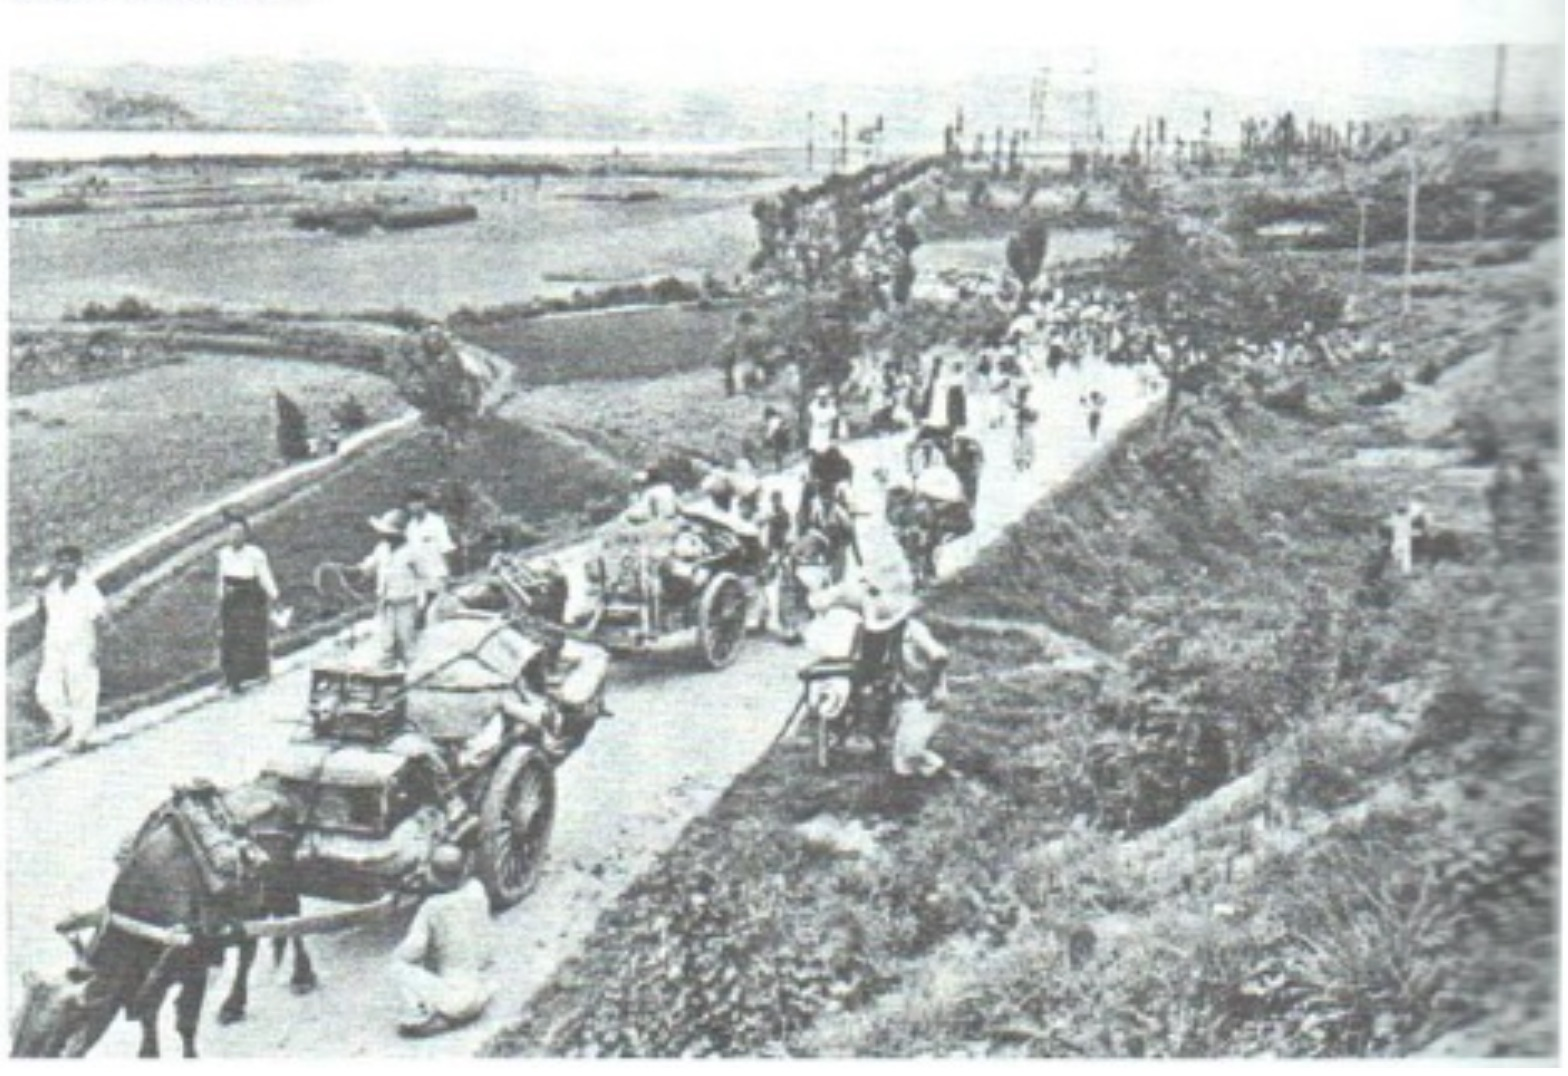
\includegraphics[width=6cm]{./Chapters/Images/02.jpg}
	\caption*{朝鲜战争中行进的难民}
\end{figure}


在15岁的时候,俊相是个瘦瘦高高,勤奋好学的男孩。从童年开始,他的数学、科学的成绩就一直是最好的。他父亲,一个失意的知识分子,对孩子们的期望很高,特别是对这个颇具天赋的长子。这也是他的梦想,期待俊相能走出这个偏远的省份,到首都平壤去念大学。如果俊相晚上9点后才回家或者功课落后了,他父亲就会迅速拿出一根专门用来教训那些不听话的孩子而准备的木棒。在整个高中期间,他要始终保持在前几名,并且通过在清津举行的长达两周的艰苦考试,才能确保能考上一流的大学,例如金日成大学。现在,俊相刚刚开始高中一年级的学业,但是他已经开始进入职业生涯的轨迹了,所有的其它事情都要为此让步,根本没时间考虑约会啊,性爱啊什么的。青春期的躁动必须静静的等待。\\

俊相试图将这些胡思乱想放到一边,在这个最关键时候,他应该集中精神学习。但是无论怎么努力,他也不能将那个留着齐耳短发跺着脚的女孩从自己的脑海里赶出去。他对她一无所知。她叫什么名字呢?她是不是真的和记忆中的一样漂亮?还是那只是记忆同他开了个玩笑?怎样才能找到她呢?\\

然而事情的发展令人吃惊,找到她的线索竟然不费吹灰之力。美兰属于那种很容易让男孩们注目的类型,仅仅是描述了她的短发就足以让俊相在他朋友的口中得到她的线索。一个同俊相一同上拳击课的男孩碰巧就她住在同一排口琴屋,相隔仅仅两个门。俊相同他攀谈起来,旁敲侧击的探听着她的消息,并让他做自己的私人耳目。邻居们悄悄议论著关于美兰和她姐姐们的闲话。人们都说她们姐妹一个比一个漂亮。她们个子都很高,这在北朝鲜是非常让人羡慕的,她们也非常有天赋。大姐擅长唱歌,另外一个姐姐画画很好。而且她们都有运动才能,排球、篮球打的都很好。这是多么美丽聪明的女孩啊!不过这些传闻的最后,总是会加上一句,只可惜他们的家庭成分太不好。\\

问题出在她们父亲的身上,一个面容憔悴,沉默寡言的矿工,同周围的邻居一样,在一个矿上工作。那是一个出产高岭土的矿,开采一种可以用于烧制陶瓷的粘土,他作为木匠,负责修理支持矿道的木支撑。关于他,我们不甚了解,唯一清楚的就是他极端自律。当其它的矿工一杯一杯豪饮着米酒的时候\footnote{有时是烧酒、朝鲜米酒,如果他们买得起的话。},美兰的父亲却滴酒不沾。他不想碰任何会让他松口谈及过去的东西。\\

美兰的父亲泰宇,于1932年出生于现在属于南韩──敌对国家的一个地方。朝鲜人通常将自己父辈的出生地视为自己的籍贯,而不论自己住的离那里有多远。泰宇出生于忠清南道,几乎在半岛的另外一侧,靠近黄海的沿岸。这是一个宁静的小村子,周围遍布翠绿的水稻田,和清津恶劣的地形完全不同的是,这里地势平坦。他的村子坐落于西山市的郊区,非常小,只有几排房子,旱地穿插于星罗棋布的水稻田中间。回到40年代,一切都是泥巴和稻草做成的,甚至是孩子们在街头巷尾踢得球也不例外。大米是这个小村庄的灵魂,是人们赖以为生的食物。种植水稻是项极其繁重的体力劳动,需要犁地、播种、插秧、全都要手工完成。在这个村子里,没有富人,但是泰宇的家在当地是数一数二的,生活比其它人过得去。但是,他们也仅仅是有个比别人大一点的茅草房而已。家里有2000坪\footnote{坪是一种朝鲜的面积单位。}左右的田地,相当于10亩。除此之外,他们家经营着一个小磨坊以贴补家用,街坊邻居们来这里把稻谷碾成白米。美兰的祖父因而也娶了两房太太,这在当时并不是什么稀罕的事情,虽然法律上只是承认第一次婚姻。泰宇是第二房太太的长子,也是家里的独子。他有两个很崇拜他的妹妹,总是跟着他屁股后面在村子里转悠,这让他十分厌烦,但是当她们慢慢出落成漂亮的姑娘时,他的朋友们却是很乐意。\\

泰宇并不是那一群孩子里年纪最大的,但是他确是天生的领袖。当男孩们玩打仗的游戏时,他总是当将军。他的朋友都叫他小拿破仑。“他很直爽又果敢,他说话很坚定,其它的人都听从他的指挥。”李钟勋,一个泰宇儿时的玩伴,这样说道。“他也非常聪明。”\\

泰宇上了小学,后来大概15岁的时候又上了中学,这在当时农民的孩子中还是比较普遍的。学校里用日语教课。日本在1910年吞并了朝鲜,废黜了朝鲜的末代国王,之后开始系统的去朝鲜化,取而代之以日本文化。在占领初期,村里的老年人被强迫剪去长辫,按朝鲜传统男性蓄发,并在头顶上挽成一个发髻,再用一顶黑帽子盖住发髻。他们被迫使用日本姓名。日本人对朝鲜人课以重税,收成的一半或更多都被掠走,日本人声称这是对他们正在进行的太平洋战争必要的支持。年轻的男男女女被船运到日本,为战争出力,女孩被逼成娼,美其名曰“慰安妇”,被迫为军队提供性服务。没有日本人的批准,他们不能做任何事情。\\

1945年8月15号这一天,日酋首裕仁\footnote{译者不愿意用“天皇”这个称呼给这个杀人魔王。}通过广播宣告日本投降。消息几天之后才传导这个小村庄。听见这个消息,男孩们冲向日本人驻扎的兵营,却发现他们已经撤走了,匆忙间连个人物品都来不及带走。占领结束了。村民们没有钱来庆祝,但他们仍兴高采烈的跑到街上,奔走欢呼,相互道贺。\\

“万岁朝鲜!”他们喜极而泣。“万岁朝鲜!”\\

朝鲜人相信他们的命运又再一次掌握在自己的手中。他们又重新收回了自己的国家。\\

当日酋首在广播里读着投降书的时候,在地球的另外一端,华盛顿特区里,两个年轻的军官,埋在一堆美国国家地理学会的地图之中,就如何处理朝鲜犯着愁。当时的华盛顿对朝鲜这个不知名的日本殖民地知之甚少。当对于德国和日本详细的战后占领计划完成的时候,只是对朝鲜做了个临时的补充。日本在朝鲜殖民统治了35年,随着他们突然的撤离,留下了一个危险的权力真空。美国担心苏联可能会占领朝鲜并以此为跳板,以便从战败的日本身上攫取更多利益。虽说在二战中是盟友,华盛顿对苏联的不信任却在与日俱增。日本宣布投降前一周,苏联的军队已经从北部进入朝鲜,而且还在继续前进。为了安抚苏联、美国人提议将北部朝鲜以一种临时托管的形式交给苏联实施管理。这两位军官,其中一位就是迪恩鲁斯特(David Dean Rusk),后来成了为美国国务卿,希望将首都首尔纳于美国的管辖之下。因此这两名军官思考着用一种简便的方式将这个半岛一分为二。最终,他们将分割线画在了北纬三十八度。\\

这条线在朝鲜的历史以及地理上都找不到任何相关的依据。朝鲜半岛像一个大拇指,从中国大陆延伸出来,这片陆地东临日本海、西临黄海、鸭绿江图们江形成了于中国的边境线。在这个半岛上,根本没有一个天然的分割线可以将它一分为二。在被日本人占领前1300年间,朝鲜都是一个统一的王国,先是由世界历史上统治时间最长的封建王朝之一的李朝统治,在李朝之前,是高丽。公元918年-1392年,高丽再之前,是半岛三国纷争的时期。缺乏一个强有力的中央政权使得这个国家四分五裂,东部地区由于其地理位置,很自然的亲日本,同样西部则倾向于中国。然而,南北的划分,则完完全全是由外国人一手炮制的,由华盛顿决定然后强加给朝鲜人的,这期间根本没有征求任何朝鲜人的意见。有传闻说,当时的美国国务卿,爱德华斯特迪纽斯(Edward Reilly Stettinius),曾询问下属,朝鲜在哪里。\\

朝鲜人对于像德国一样被分割占领感到异常愤怒。毕竟在二战里,他们不是侵略者,而是受害者。当时的朝鲜人,无奈的自嘲道“他们就是巨鲸之间的小鱼虾。”成为大国角力的牺牲品。\\

超级大国们谁都不肯让步,以成全一个统一的朝鲜。当时,朝鲜人自己内部也是派别林立,有不少是共产主义的同情者。地图上的划分很快就变成了现实。1948年,南韩成立,时年70岁的李承晚任总统,他是一个拥有普林斯顿大学博士学位的保守强硬派。随后,金日成,一个抗日英雄,在莫斯科的扶持下,也成立朝鲜民族主义人民共和国──也就是北朝鲜。北纬三十八度线,最终也成为了一个250公长,4公里宽的分割线,那里布满铁丝网、坦克陷阱、壕沟、堤防、火炮和地雷。\\

由于双方都宣称自己是代表半岛的唯一合法政府,于是战争就在所难免了。1950年6月25日星期天,拂晓之前,金日成的军队在苏联提供坦克的掩护下,潮水般越过三十八度线。他们很快就占领了首尔,并势如破竹一路向南,南韩被压缩至位于东南沿海城市釜山及其周边的狭小区域。然而,同年9月,在道格拉斯麦克阿瑟将军的指挥下,4万美军出其不意的在仁川进行了极其冒险的两栖登陆,一举改变了战局。除了美国和南韩、还有英国、澳大利亚、加拿大、法国和荷兰等15个国家加入了当时的联合国军。他们很快重新夺回了首尔、占领了平壤并且继续向北推进。然而,当联合国军迫近鸭绿江时,中国人参战了,并把他们赶了回去。随后的两年里,战事成胶着状态。到1953年7月27日,停战协议最终签署的时候,几乎300万人死于战火,整个朝鲜成了一片废墟。而战线或多或少的仍然沿着北纬三十八度线分布。即使以20世纪最牵强的战略标准来看,这都是一场无谓的战争。\\

在共产党军队入侵的时候,泰宇18岁了。他是家里的顶梁柱,妈妈妹妹都依靠着他,他父亲在战争爆发前就去世了。南韩对战争准备不足,当时军队只有65000人,大概刚刚够北朝鲜军队人数的1/4。因此政府急需征召所有身体健康的男子。有些农民对共产主义持同情态度,因为他们听说,共产党会免费分给他们土地。虽然赶走了日本人,但是他们依然穷困。然而大多数的年轻人不关心政治。“我们那个时候根本分不清派别,什么是左,什么是右。”李钟勋回忆道。但是无论什么政治信仰,他们都被南韩军队征召入伍,别无选择。\\

泰宇最后升到了军士军衔。他所在部队的最后一仗发生在金化(Kumhwa),是美军所称“铁三角”中的一角。那是一个战略位置极为重要的一个村庄,四周被群山包围着\footnote{平康和铁原构成另外两角}。那里见证了双方在战争末期最为激烈的交战,中国人试图在停火协议签订前尽可能的将战线向南推进。在1953年7月13日的晚上,3个师,大约6万人的中国军队对联合国及南韩联军发动了突然袭击;大约在晚上7:30的时候,共产党军队开始炮击联合国军阵地;晚10点左右,他们发射照明弹,“群山,村庄还有成千上万的敌人都显现在眼前。”一个美国士兵后来回忆那次战斗。军号从四面八方响起,中国军队向他们发起冲锋。“简直难以置信,那就像电影里的场景。”这位美国老兵说道。当时连下一周的大雨,爆发的山洪都被鲜血染红。\\

泰宇,此时被派到战地医疗小组,正用担架抬着一个南韩伤兵,随后,他们被中国人包围了。此时距停战协议签署仅仅两周,他和其它大约500名南韩首都师的士兵成为了战俘。\\

他作为南韩人的生涯就这么戛然而止了。美兰的父亲从来没有提及他被俘后的事情。但是可以想象到,他的待遇肯定不会比其它共产党的战俘好到哪里去。许在硕,一个逃脱的战俘,后来在回忆录\\

中写到,他们被关在肮脏的营地中,不准洗澡刷牙。头发里长满了虱子;伤员的伤口得不得任何救治,爬满蛆虫。每天只供应一顿米饭和盐水。\\

停战协议签订后,双方交换战俘,共产党方面释放了12773名战俘,其中包括7862名南韩战俘。然而还有成千上万的南韩战俘却再也没有回到家,其中包括泰宇。根据许在硕的回忆,他们在平壤火车站上了火车,原以为火车会开往南方,他们可以回家了。然而事实恰恰相反,火车向北驶去,来到中朝边境,煤炭储量丰富的山区。北朝鲜以内政部建设处的名义,在矿区附近建了新的战俘营。煤矿在北朝鲜不仅脏乱,更要命的是非常危险,矿井塌方、火灾司空见惯,时有发生。“在那里,我们战俘的命就像只苍蝇一样不值钱。”许在硕写道。“每天我走进矿井的时候,就觉得自己是一头走进屠宰场的牛,我不知道是自己还能不能活着出来。”\\

1956年,北朝鲜内阁发布一道法令,允许这些南韩战俘获得北朝鲜公民权。这就意味着最艰难的日子已经过去了,然而,另一方面,这也意味着他们永远回不了家了。对于泰宇太说,最艰难的就是在煤矿,由于贸然的开采,矿井塌方、火灾,事故不断。之后,泰宇被派到位于茂山附近的一个铁矿工作,茂山紧挨着中朝边境,位于北朝鲜一侧隶属于咸镜北道,那是一个简陋的小城。那里的工人都是前南韩人,一起住在集体宿舍里。\\

宿舍的工作人员里的有一个女孩,19岁了仍然单身──在那时候已经算是老姑娘了。她瘦骨嶙峋的因此很难称得上漂亮,然而她却有着吸引人的独特之处;她处事果敢,雷厉风行。只为了摆脱同住的妈妈和姐妹,她渴望结婚。然而,战后适龄的男性很少。因此,宿舍管理人员将她介绍给泰宇。虽然泰宇的个头并不比姑娘高,但是他说话温和,虽然浑身沾满矿井里的煤灰,却散发着绅士的气质。于是,她对这个无依无靠的年轻人顿生怜爱。当年,他们就结婚了。\\

泰宇很快就适应的北朝鲜的的生活,这对他来说很容易。朝鲜人同属一个民族,他们习惯称之为“大国家”。他们看起来完全一样。平壤口音也因为同釜山口音有着类似喉咙音而经常被取笑。连年的战乱,也让朝鲜人完全融合在了一起。出于对共产主义的恐惧,成千上万的朝鲜人穿过三八线逃往南方,其中不乏地主、商人、牧师及日据时代的通敌者。少部分共产党的认同者来到北方。不计其数没有政治立场的人们,仅仅是为了逃避战火或是北上,或是南下。\\

谁又能分清谁是北朝鲜人,而谁又是南韩人呢?婚后不久,泰宇和他的新娘就被调往位于清津附近的另一个矿山,在那里他们一个人也不认识。虽然在那里没有什么会让人对他的背景产生怀疑,然而怪异的是,在北朝鲜,总是有些人会知道。\\

战争一结束,金日成就迫不及待的开始剪除异己。他最先从对他有威胁的最高领导层开刀。他清洗了很多同他一同在中国东北进行抗日斗争的昔日战友。随后,他命令逮捕了很多朝鲜共产党南方局的创始人。他们在战争期间,发挥着至关重要的作用;现在,却是兔死狗烹的时候。整个50年代,随着更多的人被肃整,金日成在这个国家慢慢建立起类似于中国封建皇帝式的威严,至高无上,不容任何挑战。\\

在此之后,金日成腾出手来,将注意力转向普通民众。在1958年,他下令开展一项浩大的计画,试图按照政治上的可靠性,对所有北朝鲜人进行分类,雄心勃勃的想以此实现对朝鲜人的重组。当60-70年代中国的文化大革命时期,红卫兵清除“走资派”,这导致骇人听闻的混乱,邻居们相互揭发。相比之下,北朝鲜则进行的有条不紊。每个人都要进行一项有八条标准的背景审查。你的成分,即所谓的评级,要考虑你父母、祖父母、甚至旁系表亲的背景。忠诚度的调查,以各种方式进行并被冠以各种冠冕堂皇的名称。“加强党中央的指导”是第一阶段。划分成分在随后的阶段变得更加明目张胆,例如1972年至1974年的“识人计划。”\\

抛开20世纪的社会工程的术语,现在这一套就是过去朝鲜封建社会体系的一种升级,将朝鲜人完全带回了上一个世纪。在过去,朝鲜人处于一套类似于印度等级制度严苛的桎梏之下。贵族穿白衣、带黑色的马鬃高帽,而奴隶,脖子上则系着木牌子。朝鲜过去的社会等级制度受中国儒家哲学的影响极大,儒家思想认为人类社会应该严格按照金字塔一样的等级制度来划分。金日成截取了儒家思想关于人文的观点并结合以斯大林主义(Stalinism)。在金字塔的顶端不再是皇帝,而是金日成及金家。由此向下,共细分为51个阶层,归为3大类──核心阶层、动摇接触和敌对阶层。\\

敌对阶层包括妓生\footnote{女性娱乐从业者,与日本艺伎类似,能为出得起价钱的顾客提供一些特别服务。}、算命先生、巫师\footnote{在封建王朝时期,他们既是社会底层。}。敌对阶层也包括政治上的不坚定者。关于他们,在根据现居住于南韩的脱北者的证词辑写而成的北朝鲜人权白皮书上有明确定义。\\

出生富农的、商人、企业主、地主或其它私人财产被完全没收的,亲日、亲美份子、反动官僚;南方来的叛逃者……佛教徒、天主徒、被罢黜政府官员、战争期间通敌份子。\\

作为一个前南韩士兵,泰宇的成分接近这个金字塔的底部,却还不是最底层,因为还有更低的。那些人\footnote{大概总数有20万人,接近总人口1\%。}永远被关在仿照苏联古拉格\footnote{苏联的劳动集中营。}建立起来的劳动营里。在北朝鲜,成分不好的人是不允许住在橱窗式的首都平壤,或者乡村里朝南的地方,一般来说朝南的土地相对比较肥沃而且也比较暖和。泰宇是不能梦想加入劳动党的,朝鲜的劳动党类似于中国及苏联的共产党,他们把持着这些美差。\\

像泰宇这样的成分,是会被邻居们严格监视的。北朝鲜人的基层小区是按照一种叫“人民班”形式组织起来的,每个人民班大约有20户居民组成,它的职责就是是密切监视居民并管理小区的日常事务。人民班的领导由居民自行选出,通常会是一个中年妇女,她会将辖区内的任何异常情况上报给上一级政府。对于出身不好的北朝鲜人,想要改变成分几乎是不可能的事情。在这个山区省份,两江道,个人档案被锁在国家安全保卫部在当地的办公室里,并且被严密保管,以防有人企图篡改记录。在这个等级体系里,唯一的流动性是向下的。即使你处于只属于统治阶层极其亲属和党干部的核心阶层,你的成分也会因为你的不当行为而降级。一旦你有污点,它就会跟着你一辈子,永远无法摆脱。而且,就像是旧朝鲜的社会体系,家庭成分是可以继承的。父亲的罪就是儿子的罪,也是孙子的罪。\\

北朝鲜人称呼这些人为不纯──“不洁之血”也就是血统不纯。\\

美兰和她四个兄弟姐妹身上都流着这样的不洁之血。因此显而易见,他们的前途不会比他们的父亲好多少。\\

还是个孩子的时候,美兰意识不到这些在她出生之前就已经注定了的厄运。她父母认为最好不要告诉孩子们关于他们父亲出生于南韩这件事。如果孩子们知道了,因为他们的出生,他们将永远无缘于最好的学校、最好的工作,他们的人生是不是没有未来?如果这样,谁又会劳心费力的去努力学习,刻苦弹奏乐器,练习体育运动呢?\\

北朝鲜人不会被告知他们所属的阶层,因而就算家庭背景不好,负面作用也不会马上显现出来。然而孩子们却还是发现了父亲的特别之处。他有点古怪,与世无争,似乎总是背负着千斤重担。他在这里没有亲人。他不止是从不提及过去,他根本就是不说话。对所有的问题也就是回答一两个字,说话声音也总是像在耳语。当他用双手劳动,房前屋后修修补补的时候,是泰宇最开心的时刻。只有在这个时候,他可以埋头工作而不必说话。\\

现在的泰宇,完全看不出他曾是当年那个发号施令,神气活现,扮着将军的小男孩。他太太,女儿们继承了她的身高和运动天赋,则替他说了所有的话。如果孩子们要管教,如果要对邻居有所抱怨,都是她太太代他出面。如果泰宇有任何想法,他只会留在心里。偶尔,家里得到一张报纸,这在北朝鲜是很难得的,泰宇会就着家里唯一的那盏40瓦的灯泡,在昏暗灯光下静静的读着,他对于劳动党官方报纸《劳动新闻》和当地报纸《咸镜日报》上吹捧金日成最新伟大成就怎么看?他永远不会说。他相信北朝鲜的这些报导吗?他被说服了吗?\\

美兰发现他父亲对待任何事物的态度,消极被动的简直让人无法忍受。多年之后,美兰才明白那是一种求得生存的方法。仿佛是他将个性隐藏起来,以免引起对他过多的关注。在想使自己融入北朝鲜社会的数以千计的前南韩士兵中,很多人还是出了岔子。美兰的母亲后来告诉她,他父亲有四个与他一同在煤矿工作的南韩伙伴,就因一点点的过失都被处决了,尸体被草草的扔到万人坑里。作为敌对阶层中一员,怀疑是徒劳的,因为你永远不能从中获益。任何影射金日成的嘲讽或者对南韩的思乡之情,都会给你带来极大的麻烦。特别是谈论朝鲜战争和关于谁先发动战争的话题简直就是禁忌。官方的历史\footnote{在北朝鲜也只有官方的历史。},声称战争是南韩军队在美国的命令下挑起的,而不是北朝鲜的军队暴风般的越过三八线。“美国帝国主义指使李承晚傀儡集团挑起朝鲜战争。”援引朝鲜《劳动新闻》。然而,每一个记得1950年6月25号发生了什么的人\footnote{哪一个朝鲜人又能忘记呢?}都心知肚明,只有明智点把嘴闭上。\\

随着孩子们一天天的长大,父亲出生给他们所带来的影响也就日益凸显出来。到15岁的时候,义务教育结束,学生们开始申请高中。那些没有机会晋升的人就会分配去工作单位,可能是工厂,也可能是煤矿,或者类似的地方。但是美兰的姐姐们非常自信,她们能得到进一步深造的机会。他们如此聪明,长得又漂亮,也非常活跃,老师同学们都非常喜欢她们。如果她们不是如此优秀,被拒绝可能就是顺理成章的事情了。\\

她的大姐,美熙,天生一副好嗓子。无论唱温柔婉约的朝鲜民歌,还是歌颂金日成的赞歌,邻居们都会过来聆听。她也经常被邀请参加各种公开演出。歌唱是北朝鲜非常重视的一项才能,因为没什么人有立体声音响。美熙也非常漂亮,曾经有一个画家专程跑来画她的素描肖像。她自己也十分期待能有机会到高等艺术学校去深造。当得知被拒绝之后,她一连哭了好几天。她们的母亲,是一定知道内在原因的,即便如此,她还是跑去找校长讨个说法,校长很是同情她们,但也是无能为力。她解释道,只有成分好的学生才有资格进入表演艺术学校。\\

美兰没有什么特殊的艺术、运动才能,但是她是一个好学生,而且长得也很漂亮。在她15岁那一年,学校里突然来了一群穿着深色衣服的人,男男女女看上去都不苟言笑。他们是Okwa,来自劳动党中央第五部的选拔人员,在全国范围内,选拔年轻女性作为金日成和金正日的随身侍从。如果被选中,姑娘们将被送到一个训练营进行军事化训练,之后就会被派往领导人遍布全国的住地。一旦被录取,她们就不能回家,但是她们的家人将得到贵重的礼物作为补偿。这些女孩们具体做什么,外界不得而知。有人说是做秘书,服务员,或者演员;也有谣传说是给领导人做情妇。所有的这些都是美兰从一个朋友那里听来的,朋友的表姐就曾被选中。\\

“你知道,金正日、金日成也是凡人,和普通人一样他们也有七情六欲。”美兰的朋友耳语道。美兰似懂非懂的点着头,不好意思的承认她根本没听明白话里的意思。像她这么大年纪的北朝鲜的女孩,根本不知道情妇是什么意思,他们只是觉得能服务于领袖那是莫大的光荣。只有最聪明,最漂亮的女孩才会被选中。\\

当这些选拔者走进教室的时候,学生们都坐直身体,安静的等待。女孩子们两个人一桌,排成长长的一排。美兰当时身上穿着校服,脚下是一双帆布运动鞋。选拔者在课桌之间来回穿行,不时的停下来仔细打量。当来的美兰的课桌前时,他们的脚步慢了下来。\\

“你,站起来。”一个选拔者命令。示意她跟着他们到了教师的休息室。当她到哪里时,发现还有四个女孩等在那里。在教师休息室里,他们看了她的档案,给她量了身高。160厘米,美兰是当时班上最高的女孩。他们还不断的问她一些问题,例如:她的成绩怎么样?她最喜欢那门课?她的健康状况怎么样?身体上有没有疤痕?美兰十分冷静的一一作答,并且认为她的回答是合适的。\\

之后就杳无音信了。美兰并不想真的被他们从父母身边带走,但是被拒绝总是件令人痛苦的事情。\\

自那时起,孩子们也慢慢意识到他们的家庭背景可能有问题。他们开始怀疑他们的父亲是不是来自从国界的另外一边,但是,是在什么情况下呢?他们设想父亲应该是一名坚定的共产党员,英雄般的离开南韩,加入金日成的军队。美兰的弟弟最终迫使事实浮出水面。锡柱是一个总是皱着眉头的充满活力的年轻人,他曾经花了几个月的时间来准备一所师范学校的录取考试。他完全知道每一道题的正确答案。当被告知未通过考试的时候,他愤怒的找到了考官讨要一个说法。\\

事实是灾难性的。孩子们常年来被灌输以北朝鲜所书写的历史。美国人就是恶魔的化身,南韩就是美国人可怜的马前卒。照片上,他们的家园被美国人的炸弹炸成一片焦土。文章里,美国及南韩士兵冷笑着将刺刀插入无辜百姓的身体里。课本上,连篇累牍的述说着人们被敌人火烧、碾压、刀刺、射杀、关押的故事。现在,他们知道了他们的父亲,曾是一个为美国佬助纣为虐的南韩士兵,事实让人无法接受。锡柱人生里第一次喝醉了。他离家出走,住到了一个朋友的家,直到2周后,朋友才将他劝回了家。\\

“你要知道他终究是你的父亲啊”朋友力劝他。这句话深深的触动了锡柱。他知道他像其它的朝鲜男孩一样,特别是作为家里的独子,他必须尊重他的父亲。锡柱回到了家,跪地请求父亲的原谅。他第一次看到父亲老泪纵横。\\

当孩子们慢慢发现父亲的真相时,他们几乎是最后知后觉的。街坊邻居早就传开了泰宇层是南韩士兵,并且人民班已被通知对他们家要保持警惕。俊相几乎在得到他在剧院外邂逅女孩的名字的同时,他就听说了这个传言。俊相非常清楚和这样家庭出生的女孩联系过密会毁了他的前程。他不想退缩,但是,按照儒家思想的传统,如同所有北朝鲜人一样,他是个背负了使命的孩子。他相信他来到这个世上注定是要侍从他父亲的,而他父亲的愿望就是,希望他能考入平壤的大学。他需要的不仅仅是最高的分数,而是操行上也必须无懈可击。哪怕是一丁点的不小心,都有可能会毁了他,因为他自己的家庭成分也是有问题的。\\

俊相的父母都是出生于日本的朝侨,二战结束的时候,在日本几乎有200万的朝侨。这些朝鲜人的小社会是朝鲜和日本的一个交集,主要构成是:来日本求学的朝鲜精英,战争期间,因战争需要被强行征召的人,以及劳工。尽管他们当中,有些人富了起来,他们始终是少数民族,处处遭日本人的冷眼。他们渴望能回到祖国,但是问题是,那一个是祖国?在朝鲜半岛处于分裂状态,在日朝鲜人也分为两派,一派支持南韩,一派同情北朝鲜。亲北朝鲜的人成立了“朝总联”──在日朝鲜人总联合会。\\

对一些民族主义者来说,北朝鲜更像是祖国,至少在过去北朝鲜同日本人的殖民统治做着坚决的斗争,反观李承晚的亲美政府,居然重用这许多日据时代的通敌者。而且在60年代,北朝鲜的经济发展看上去也远比南韩来的强劲。北朝鲜的宣传机器也使出浑身解数,一张张海报显示着这个新生的国家在金日成的英明领导下,一切都那么欣欣向荣,面色红润的孩子们在操场上玩耍,崭新的农用设备在广袤的田野里收获着丰收。时至今日,人们丝毫不会去理会这些拙劣的、带明显社会主义色彩的宣传手法,然而在当时,他们辅以事实证明,以至很多人都被说服。\\

总共超过8万人掉入这个陷阱,俊相的祖父就是其中一个,俊相的祖父是日本共产党党员,因为其左翼信仰,还曾在日本坐过牢。由于自认为太老、太弱,他将他的长子送回到北朝鲜,代替他实现建设新国家的心愿。1962年,渡船经过21个小时的航行之后横跨日本海,俊相的父亲登上了北朝鲜这片陌生土地。因为是个工程师,属于当时北朝鲜急需的人才,俊相的父亲很快被派往位于清津的工厂。几年之后,在那里,俊相的父亲遇到了同为朝侨的一位举止优雅的姑娘,她与她父母在和他几乎差不多的时间从日本抵达北朝鲜。俊相的父亲相貌平平,有着一个溜肩,而且皮肤还疙疙瘩瘩的,虽然其貌不扬,但是却知识渊博,十分有学问。家里人都说,他看上去像个土匪,说起话来却是个诗人。凭着一腔热忱和锲而不舍的精神,他终于如愿以偿,抱得美人归,她最终同意了他的求婚。\\

俊相的父母总能弄到些钱,使他们的生活始终比大多数的北朝鲜人要好。他们想方设法弄到一套独门独院的房子──这在北朝鲜可是非常稀罕的,因为在院子里开辟个小花园,就可以种些菜。在90年代之前,北朝鲜人是不允许留有自留地的。房间里摆放着五个木制大橱柜。里面存放着产自日本的棉被和衣物\footnote{朝鲜人晚上睡在地板上的垫子上,那是一种亚洲传统的就寝方式,早晨起床后,就把卧具卷起置于橱柜内。}。北朝鲜人,如果要判断一个人的家境如何,只需要看看他家有几个橱柜就可以了,俊相家有五个大橱柜,也就是说家境是非常殷实的了。不仅如此,俊相家的家用电器也比邻居们多,有电扇、电视、缝纫机、8声道的放音机、照相机、甚至还有冰箱,这在北朝鲜是个非常罕有之物,因为人们根本没有什么多余的食物需要冷藏保鲜。\\

然而,更不寻常的是,俊相家居然还养有宠物,一条朝鲜种的丰山犬──一种全身长满雪白长毛的狗有点类似于波美拉尼亚丝毛狗。虽然在乡下,一些北朝鲜人也养狗,但是那是把狗当成一种家畜,养它们主要是用来做“补身汤”,那是一种很辣的用狗肉来熬炖的汤。把狗当成家庭宠物来养,简直闻所未闻。谁负担的起这多出来的一张嘴呢?\\

事实上,日籍朝鲜人,也被称为Kitachosenjin,从日本回到北朝鲜后,又被称为Kita-Chosen,有他们着自己的圈子。他们有这独特的口音,也倾向于相互通婚。虽然以日本的生活标准来看,他们远称不上富足,但是相比于普通的北朝鲜人来说,他们的生活已经属于上等的了。他们来到这个新国家的时候,脚下蹬着皮鞋,身上穿着羊毛衫,而北朝鲜人那时只是穿着帆布鞋和闪闪发亮的人造纤维。他们在日本的亲属也会定期的寄来一些日元,这让他们可以在只收硬通货的特供商店里买到家电。甚至有些人还买了车,然而很快就因为买不到零配件而开不动了,最后不得不将其捐给北朝鲜政府。尽管来了很多年了,很多亲属仍然会带着钱和礼物乘坐万景峰92号轮渡定期的来看望这些朝侨。渡轮是由亲北朝鲜的“朝总联”运营的,它的定期到访也是受北朝鲜官方所支持的,因为这可以为这个国家带来宝贵的外汇。朝侨亲属们带来的钱,最终都会落到政府的口袋里。尽管经济状况比较好,这些朝侨在朝鲜的社会等级却是很低的。不论你是不是因为拥护共产党,而放弃日本舒适的生活而来到北朝鲜,你都会被划归为敌对阶层。这个政权不相信那些有钱的但是却不是劳动党党员的人。他们也是北朝鲜人中少数被允许同外界有联系的人,然而此举也意味着他们很不可靠;因为,这个政权的力量就来自于将自己的民众完全同外界隔绝起来的能力。\\

这些新移民很快就从他们的理想主义的幻想中清醒过来。有些早期的移民写信给家人,发出警告,让其它人不要继续前来,但是这些信件都被截获进而被销毁。很多朝侨,有些甚至是“朝总联”的骨干在70年代早期的肃整中被处决,家人被投入劳动集中营。\\

俊相偶尔听到父母耳语这些事情。当他们要来抓你的时候,事先没有任何迹象。突然,半夜里卡车就停在屋子外面,你只有1-2个小时收拾收拾家当。当俊相听见这些的时候,非常害怕,而且这些事情也很隐秘,不好细说。然而这些事情又是实实在在时有发生的。因此俊相天生说话就很小心谨慎。\\

俊相也十分低调,以避免激起他人的嫉妒。他穿着日本产的厚羊毛袜,而大多数其它的孩子根本就没有袜子穿,于是他把总是拉长裤腿把脚罩住,避免引起其它人的注意。后来他说他自己就像一个敏感的小动物,终日提心吊胆,时时刻刻竖起耳朵,警惕着四周的捕食者。\\

即使有着这些暖和的毛衣、家电、毯子什么的,可是俊相家的日子比美兰家的也安逸不到哪里去。俊相的母亲,离开日本时还是个无忧无虑人见人爱的漂亮女孩,随着年龄的增长,青春的逝去,也变得越来越忧郁。在生了4个孩子之后,她的身体再也没有恢复。晚上,俊相的父亲也总是枯坐着,抽着闷烟,长吁短叹。他们并不害怕被其它人听见──独门独户的好处就是还能有些隐私──而是,他们不敢说出真实的想法感受。他们不能跑出去说,他们想离开社会主义的天堂,回到资本主义的日本。\\

家里天天被一种无法言述的气氛笼罩着:每过去一天,就更深一步的认识到来到朝鲜这个决定是多么可怕的一个错误。他们意识到想回日本是不可能的了,他们必须在逆境中求发展。解救家庭的唯一方式就是融入这个体系,伺机爬到塔顶。家庭的希望就寄托在俊相的身上。只有他进入平壤读大学,他才有可能加入劳动党,到那时家里的日本资产阶级的色彩才可能被宽恕。旷日持久的巨大压力,让俊相时时处于紧张,也形成他犹犹豫豫的性格。他迷恋着那天在剧院外碰见的女孩,也思讨着如何接近她,然后最终的结果确是,什么都没做。\\
